\documentclass{beamer}
\usepackage{amsmath}
\usepackage{amssymb}
\usepackage{pgf}
\usepackage{tikz}
\usepackage{listings}
\usepackage{color}
\usetikzlibrary{matrix}
\usetheme{boxes}
\newcommand{\fig}{./figures} % common figure path
\newcommand{\msin}{\mbox{sin}} % math sin
\newcommand{\mcos}{\mbox{cos}} % math sin
\newcommand{\dbbslsh}{\textbackslash \textbackslash} % common figure path
\newcommand{\frnzplt}{FranzPlot }
\DeclareMathSymbol{\shortminus}{\mathbin}{AMSa}{"39}
\newenvironment{myblock}[3]{%
\definecolor{smtbx}{rgb}{0.64,0.76,0.68}
\setbeamercolor{block body}{#2}
\setbeamercolor{block title}{#3}
\begin{block}{#1}}{\end{block}}
\title[Curve e Sup. - Lab 8]{Curve e Superfici per il Design \\ Laboratorio 8 - Curve di Bezier 2}
\author[Prof. Parolini]{Prof. Nicola Parolini}
%\institute[dimat]{Long Inst.}
\date{12 Dicembre 2019}

\begin{document}
%\lstset{language=POV}
\begin{frame}
\maketitle
\end{frame}
\section{Introduzione}

\begin{frame}
\frametitle{Materiali}
Il materiale per l'esercitazione di oggi:
\begin{itemize}
\item Questa presentazione \\ (\texttt{Materiale Didattico/Laboratori/lab 8/lab8\_testo.pdf});
\item Il file trasformazioni\_ref.pdf 
\item La cartella \texttt{Materiale Didattico/Laboratori/lab 8/consegna} su cui caricare il file \texttt{.toml} risultante del primo esercizio.
\item L'eseguibile del \frnzplt \\ (\texttt{Software/Franzplot 19.08 - Windows.exe})
\end{itemize}
\end{frame}

%
\begin{frame}
\frametitle{Curve di Bezier di ordine 2}
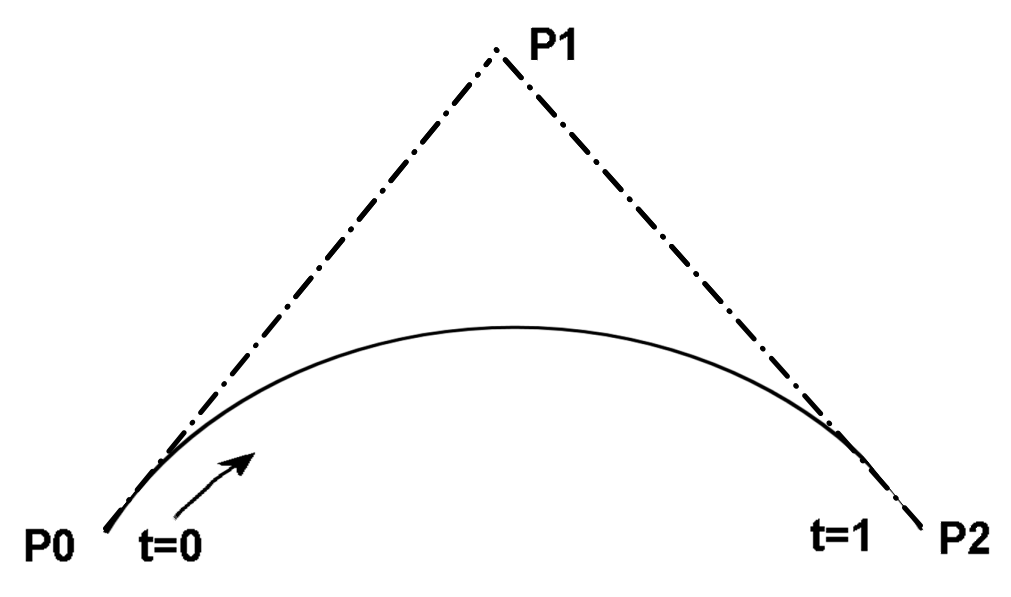
\includegraphics[width = 0.4\textwidth]{\fig/bez2.png}
\begin{displaymath}
\mathbf{x} = (1-t)^2\mathbf{p}_0 + 2t(1-t)\mathbf{p}_1 + t^2 \mathbf{p}_2
\end{displaymath}
%
\begin{myblock}{}{bg=smtbx,fg=black}{bg=smtbx, fg=red}
\begin{itemize}
\item Tangente in $t=0$: $2(\mathbf{p}_1-\mathbf{p}_0)$
\item Tangente in $t=1$: $2(\mathbf{p}_2-\mathbf{p}_1)$
\end{itemize}
\end{myblock}
\end{frame}
%
\begin{frame}
\frametitle{Curve di Bezier di ordine 3}
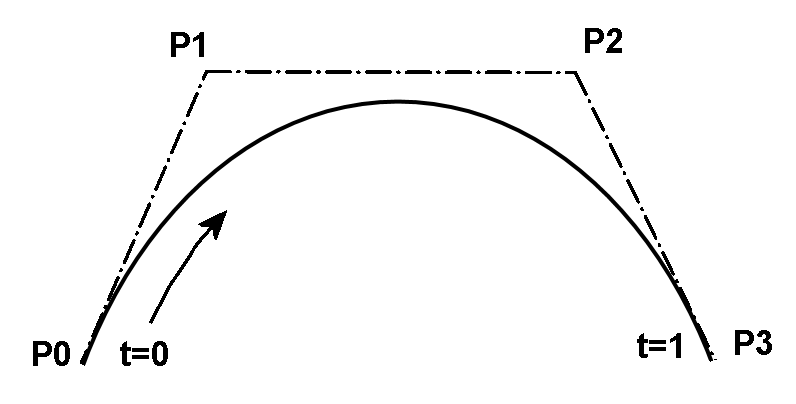
\includegraphics[width = 0.4\textwidth]{\fig/bez3.png}
\begin{displaymath}
\mathbf{x} = (1-t)^3\mathbf{p}_0 + 3 t(1-t)^2\mathbf{p}_1 + 3 t^2(1-t) \mathbf{p}_2+ t^3 \mathbf{p}_3
\end{displaymath}
\begin{myblock}{}{bg=smtbx,fg=black}{bg=smtbx, fg=red}
\begin{itemize}
\item Tangente in $t=0$: $3(\mathbf{p}_1-\mathbf{p}_0)$
\item Tangente in $t=1$: $3(\mathbf{p}_3-\mathbf{p}_2)$
\end{itemize}
\end{myblock}
\end{frame}
%
%% %%%% Raccordo tra le curve
\begin{frame}
\frametitle{Raccordo tra curve di Bezier - i}
Data una curva definita dai punti $P_0 \dots P_3$ e dal parametro $t$ e una curva definita dai punti $Q_0 \dots Q_3$ e dal parametro $s$, vediamo quali sono
    le relazioni che legano le tangenti delle due curve quando vogliamo che il raccordo sia liscio ($C^1$). Abbiamo 4 casi:
\begin{columns}
\begin{column} {0.49\textwidth}

\begin{itemize}
\item Se $\mathbf{p}_0 \equiv \mathbf{q}_3 \Rightarrow t=0$, $s = 1$;
 $3(\mathbf{p}_1-\mathbf{p}_0) = 3(\mathbf{q}_3-\mathbf{q}_2)$ (\textbf{Caso A});
\item Se $\mathbf{p}_3 \equiv \mathbf{q}_0 \Rightarrow t=1$, $s = 0$;
 $3(\mathbf{p}_3-\mathbf{p}_2) = 3(\mathbf{q}_1-\mathbf{q}_0)$ (\textbf{Caso B});
\end{itemize}
\end{column}
\begin{column} {0.49\textwidth}
\begin{itemize}
\item Se $\mathbf{p}_0 \equiv \mathbf{q}_0 \Rightarrow t=0$, $s =0$;
 $3(\mathbf{p}_1-\mathbf{p}_0) = -3(\mathbf{q}_1-\mathbf{q}_0)$ (\textbf{Caso C});
\item Se $\mathbf{p}_3 \equiv \mathbf{q}_3 \Rightarrow t=1$, $s = 1$;
 $3(\mathbf{p}_3-\mathbf{p}_2) = -3(\mathbf{q}_3-\mathbf{q}_2)$ (\textbf{Caso D});
\end{itemize}
\end{column}
\end{columns}
\vspace{0.6cm}
\textbf{Nota 1: nei casi C e D la connessione \`e liscia ma abbiamo un cambio di segno della tangente!}
\vspace{0.3cm}

    \textbf{Nota 2: in caso di curva di ordine 2 la logica resta identica, cambiano solo le espressioni delle derivate}
\end{frame}
%
\begin{frame}
\frametitle{Raccordo tra curve di Bezier - ii}
\begin{columns}
\begin{column}{0.6\textwidth}
\begin{tikzpicture}
\node[anchor=center, inner sep = 0](image)at (0,0) {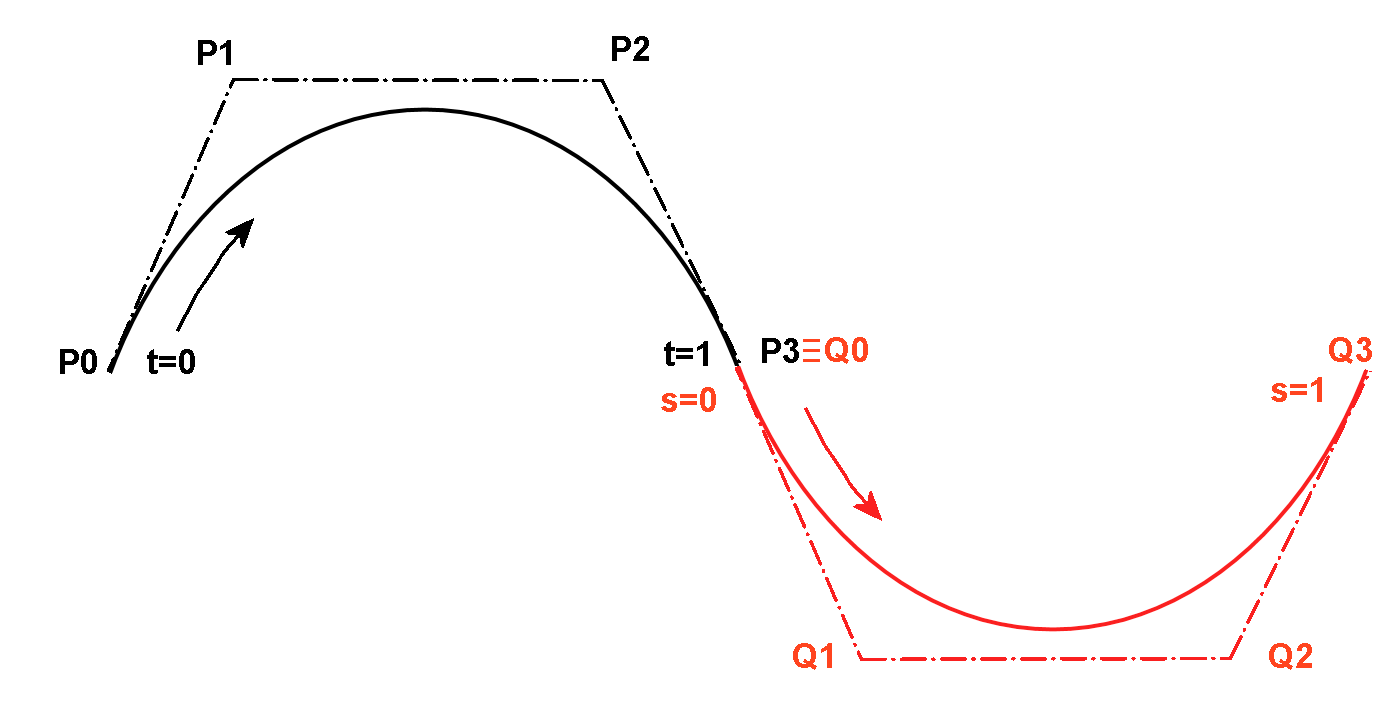
\includegraphics[width=\textwidth]{\fig/bezcon_A.png}};
\node[align=center,blue,font={\bfseries}] at (image.north west) {Caso B};
\end{tikzpicture}
\end{column}
\begin{column}{0.3\textwidth}
\begin{tikzpicture}
\node[anchor=center, inner sep = 0](image)at (0,0) {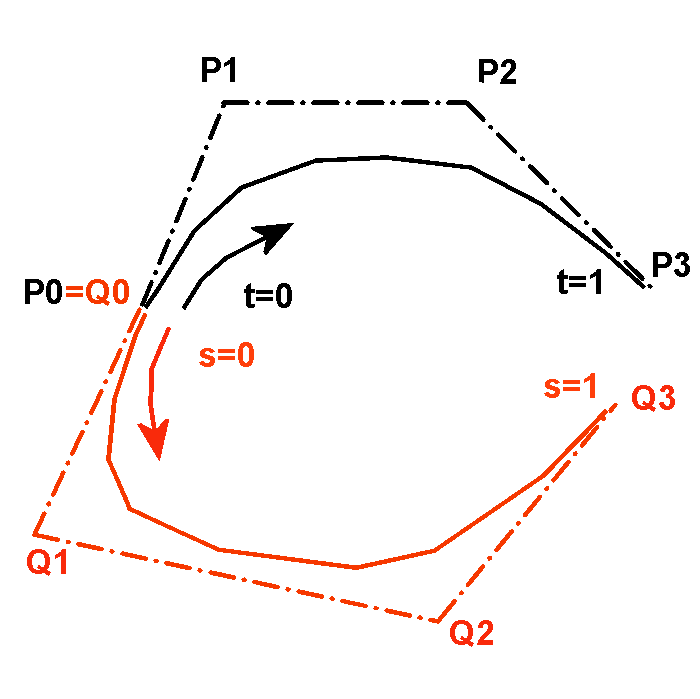
\includegraphics[width=\textwidth]{\fig/bezcon_C.png}};
\node[align=center,blue,font={\bfseries}] at (image.north west) {Caso C};
\end{tikzpicture}
\end{column}
\end{columns}
\begin{columns}
\begin{column}{0.3\textwidth}
\begin{tikzpicture}
\node[anchor=center, inner sep = 0](image)at (0,0) {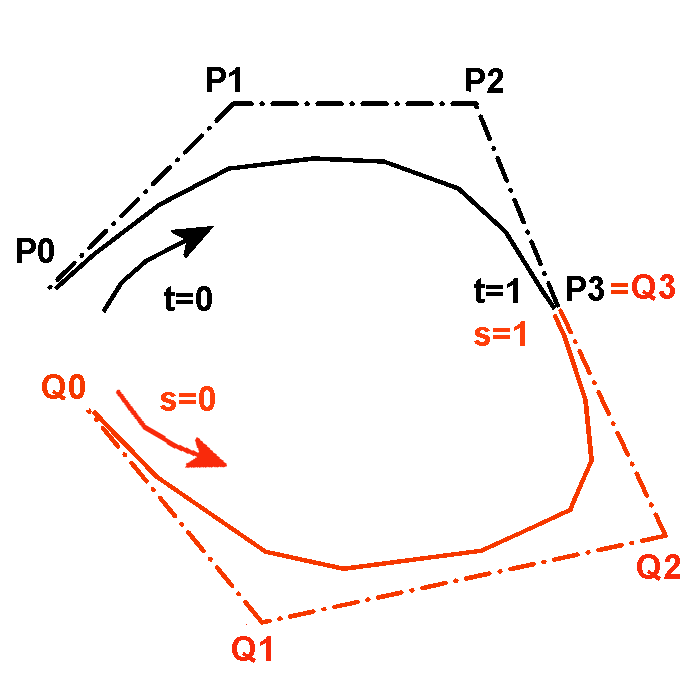
\includegraphics[width=\textwidth]{\fig/bezcon_D.png}};
\node[align=center,blue,font={\bfseries}] at (image.north west) {Caso D};
\end{tikzpicture}
\end{column}
\begin{column}{0.6\textwidth}
\begin{tikzpicture}
\node[anchor=center, inner sep = 0](image)at (0,0) {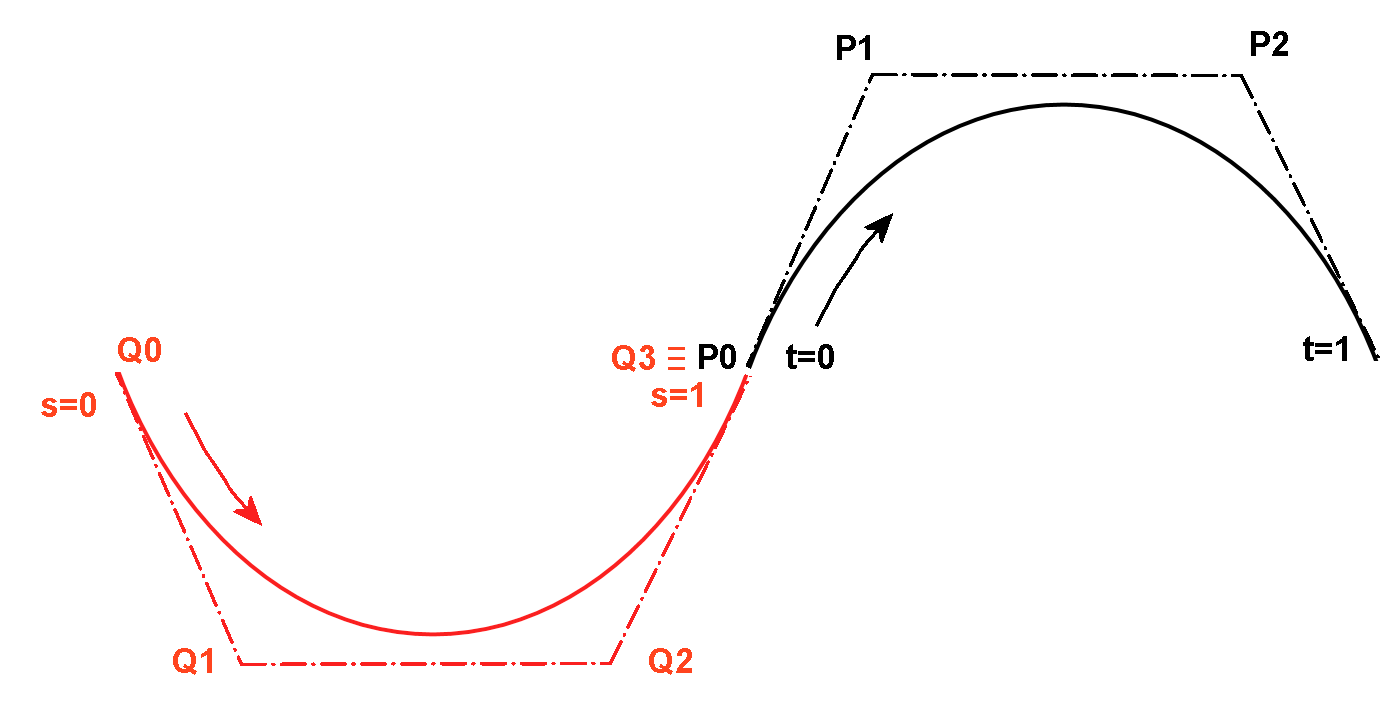
\includegraphics[width=\textwidth]{\fig/bezcon_B.png}};
\node[align=center,blue,font={\bfseries}] at (image.south east) {Caso A};
\end{tikzpicture}
\end{column}
\end{columns}
\end{frame}

%
\begin{frame}
\frametitle{Esercizio 1}
\begin{itemize}
\item Rappresentare in \frnzplt le due curve di Bezier i cui punti di controllo siano:
\begin{align*}
    P_0 &= (0,0,0) \quad & Q_0 &= (2, 0, 1)\\
    P_1 &= (1,0,3) \quad & Q_1 &= (3, 0, -1)\\
    P_2 &= (2,0,1) \quad & Q_2 &= (3, 0, 1)
\end{align*}
\item Calcolare i vettori $\overrightarrow{P_1 P_2}$ e $\overrightarrow{Q_0 Q_1}$, e rappresentarli spiccandoli rispettivamente
    dai punti $P_1$ e $Q_0$.
\item Cosa possiamo dire riguardo al raccordo delle due curve di Bezier?
                \item Salvare la scena ottenuta in un file \texttt{toml} e caricarlo sulla seguente cartella di Beep: \\
                    \texttt{Materiale Didattico/Laboratori/lab 8/consegna}
\end{itemize}
\end{frame}
%
\begin{frame}
\frametitle{Esercizio 1 - i}
    \begin{itemize}
        \item Svolgiamo i calcoli e notiamo che i due vettori sono uguali:
    \begin{displaymath}
        \overrightarrow{P_1 P_2}
        = \begin{bmatrix} 2 \\ 0 \\ 1\end{bmatrix} - \begin{bmatrix} 1 \\ 0 \\ 3\end{bmatrix}
        = \begin{bmatrix} 1 \\ 0 \\ -2 \end{bmatrix}
            \quad
        \overrightarrow{Q_0 Q_1}
        = \begin{bmatrix} 3 \\ 0 \\ -1\end{bmatrix} - \begin{bmatrix} 2 \\ 0 \\ 1\end{bmatrix}
        = \begin{bmatrix} 1 \\ 0 \\ -2 \end{bmatrix}
    \end{displaymath}

    \item Le due curve si raccordano in $P_2 \equiv Q_0$. Guardando la casistica illustrata in precedenza, vediamo subito che
    ci troviamo nel \textbf{caso B}. Le curve sono di grado 2, quindi la relazione che dobbiamo verificare sar\`a:
    \begin{align*}
        2(P_2-P_1) &= 2(Q_1-Q_0) \\
        &\Downarrow \\
        P_2-P_1 &= Q_1-Q_0
    \end{align*}
            Che \`e proprio il calcolo dei due vettori fatti in precedenza, pertanto il raccordo \`e liscio ($C^1$).

    \end{itemize}
\end{frame}

\begin{frame}
\frametitle{Esercizio 1 - ii}
        Quando le curve da raccordare hanno \textbf{lo stesso grado} non \`e necessario confrontare le tangenti delle curve!
        \vspace{0.5cm}

        Infatti se il grado \`e lo stesso tutti e 4 casi si riconducono al confronto di due vettori:
    \begin{itemize}
        \item Chiamiamo $\overrightarrow v$ il vettore che va dal \textbf{punto di raccordo} al \textbf{punto di controllo adiacente} della seconda curva\\
            ($\overrightarrow{Q_0 Q_1}$ in questo esercizio, rosso in figura)
        \item Chiamiamo $\overrightarrow u$ il vettore che va dal \textbf{punto di controllo adiacente} della prima curva al \textbf{punto di raccordo}\\
            ($\overrightarrow{P_1 P_2}$ in questo esercizio, verde in figura)
        \item Allora il raccordo sar\`a liscio se e solo se $\overrightarrow u = \overrightarrow v$.

    \end{itemize}
\end{frame}

\begin{frame}
\frametitle{Esercizio 1 - iii}
\begin{center}
\includegraphics[width=0.62\textwidth]{\fig/lab8_es1_scene.png}
\end{center}
\end{frame}


\begin{frame}
\frametitle{Esercizio 2}
\begin{itemize}
\item Siano date le due curve di Bezier i cui punti di controllo siano:
\begin{align*}
    P_0 &= (0,0,0) \quad & Q_0 &= (-2, 0, 1)\\
    P_1 &= (1,1,0) \quad & Q_1 &= (-2, -2, 1)\\
    P_2 &= (2,1,1) \quad & Q_2 &= ? \\
    P_3 &= (1,2,0) \quad & Q_3 &= (0, 0, 0)
\end{align*}
con $Q_2$ inizialmente incognito.
\item Determinare il grado della prima curva e scriverne la parametrizzazione.
\item Le due curve si raccordano? Se s\`i, in quali punti?
\item Calcolare la tangente della prima curva in $P_0$.
\item Vogliamo imporre che il raccordo tra le due curve sia liscio (raccordo $C^1$). Sfruttando le informazioni calcolate al punto precedente,
    determinare $Q_2$.
\end{itemize}
\end{frame}

\begin{frame}
	\frametitle{Esercizio 2 - i}
	\begin{itemize} 
		\item Numero punti di controllo = 4 \ $\Rightarrow$ \ Ordine curva = 3.
		\begin{displaymath}
		\mathcal{B}(t) = (1-t)^3\mathbf{p}_0 + 3 t(1-t)^2\mathbf{p}_1 + 3 t^2(1-t) \mathbf{p}_2+ t^3 \mathbf{p}_3
		\end{displaymath}
		\begin{displaymath}
		= (1 - t)^3 \begin{bmatrix} 0 \\ 0 \\ 0 \end{bmatrix} +
		  3t(1-t)^2 \begin{bmatrix} 1 \\ 1 \\ 0 \end{bmatrix} + 
		  3t^2(1-t) \begin{bmatrix} 2 \\ 1 \\ 1 \end{bmatrix} +
		        t^3 \begin{bmatrix} 1 \\ 2 \\ 0 \end{bmatrix}
		\end{displaymath}

                \vspace{0.5cm}
            \item Le curve si raccordano in $P_0 \equiv Q_3$, ma essendo $Q_2$ incognito non possiamo
        ancora dire se il raccordo sia liscio o no.
	\end{itemize}
\end{frame}

\begin{frame}
	\frametitle{Esercizio 2 - ii}
	\begin{itemize} 
		\item Il punto $P_0$ \`e il punto in cui la curva di Bezi\`er inizia, ovvero il punto che abbiamo quando $t=0$: $P_0 = \mathcal B (0)$. \\
                    La tangente in $t=0$ per la nostra curva (grado 3) \`e:
                    \begin{align*}
                        \overrightarrow v = 3(P_1 - P_0) \quad \Rightarrow \quad \overrightarrow v = \begin{bmatrix} 3 \\ 3 \\ 0 \end{bmatrix}
                    \end{align*}
            \item Le curve si raccordano in $P_0 \equiv Q_3$, quindi siamo nel \textbf{caso A}.
                Per avere un raccordo $C^1$, la tangente in $Q_3$ deve essere uguale alla tangente in $P_0$:
                    \begin{align*}
                        3(Q_3 - Q_2) = \overrightarrow v \quad \Rightarrow Q_2 = Q_3 -\frac{1}{3} \overrightarrow v = \begin{bmatrix} -1 \\ -1 \\ 0 \end{bmatrix}
                    \end{align*}
	\end{itemize}
\end{frame}

\begin{frame}
	\frametitle{Esercizio 2 - iii}
	\begin{itemize} 
		\item In alternativa, visto che le curve sono entrambe di grado 3, possiamo usare il metodo di confronto dei vettori usato nell'esercizio precedente: \\
                    per avere un raccordo $C^1$, vogliamo imporre che $\overrightarrow {Q_3 Q_2} = \overrightarrow{P_1 P_0}$.
                    \begin{gather*}
                        Q_2 - Q_3 = P_0 - P_1 \\
                        Q_3 \equiv P_0 \quad \Rightarrow \quad Q_2 = 2P_0 - P_1 \\
                        Q_2 = 2 \begin{bmatrix} 0 \\ 0 \\ 0 \end{bmatrix} - \begin{bmatrix} 1 \\ 1 \\ 0 \end{bmatrix} = \begin{bmatrix} -1 \\ -1 \\ 0 \end{bmatrix}
                    \end{gather*}
	\end{itemize}
\end{frame}

%\section{Esercizi}
\begin{frame}
\frametitle{Esercizio 3}
Sia data la curva di Bezier determinata dai punti
\begin{align*}
P_0 &= (0,0,0 ) \\
P_1 &= (1,0,0 ) \\
P_2 &= (2,0,2 )
\end{align*}
Si determini una nuova curva di Bezier tale che:
\begin{itemize}
\item Il punto $Q_0$ coincida con $P_0$;
\item Il punto $Q_1$ sia tale che le due curve abbiano un raccordo liscio;
\item Il punto $Q_2$ sia ottenuto come riflessione del punto $P_2$ rispetto al piano
    passante per l'origine e avente \textit{vettore} normale $[-1, 1, 0]^T$.
\item Rappresentare le due curve in \frnzplt
\end{itemize}
\end{frame}

\begin{frame}
	\frametitle{Esercizio 3 - i}
	\begin{itemize} 
            \item Come sempre, possiamo guardare le tangenti (stavolta siamo nel \textbf{caso C}) \\ 
                \begin{centering}
                oppure\\ 
                \end{centering}
                
                \vspace{0.25cm}
                
            \item imporre l'uguaglianza dei due vettori.
            \begin{itemize} 
                \item Per la seconda curva, il raccordo \`e in $Q_0$, il punto di controllo adiacente \`e $Q_1$ \\
                    $\quad \Rightarrow$ prendo il vettore $\overrightarrow {Q_0 Q_1}$.
                \item Per la prima curva, il raccordo \`e in $P_0$, il punto di controllo adiacente \`e $P_1$\\
                    $\quad \Rightarrow$ prendo il vettore $\overrightarrow {P_1 P_0}$.

                \item Impongo $\overrightarrow {P_1 P_0} = \overrightarrow {Q_0 Q_1}$:
                    \begin{gather*}
                        Q_1 - Q_0 = P_0 - P_1, \quad Q_0 \equiv P_0 \quad \Rightarrow \quad Q_1 = 2P_0 - P_1 \\
                        Q_1 = 2 \begin{bmatrix} 0 \\ 0 \\ 0 \end{bmatrix} - \begin{bmatrix} 1 \\ 0 \\ 0 \end{bmatrix} = \begin{bmatrix} -1 \\ 0 \\ 0 \end{bmatrix}
                    \end{gather*}
            \end{itemize}
	\end{itemize}
\end{frame}

\begin{frame}
\frametitle{Esercizio 4}
Sia data la curva di Bezier $\mathcal B$ determinata dai punti
\begin{align}
P_0 &= (1,2,0 )\nonumber\\
P_1 &= (1,2,2 )\nonumber\\
P_2 &= (1,0,2 )\nonumber
\end{align}
\begin{itemize}
\item Determinare l'ordine della curva e scriverne la rappresentazione parametrica.
\item Ottenere una nuova curva applicando a $\mathcal B$ una rotazione di 90 gradi intorno l'asse $x$.
\item Rappresentare le due curve in \frnzplt
\item Cosa possiamo dire sul raccordo tra le due curve?
\end{itemize}
\end{frame}
%
%
\begin{frame}
\frametitle{Esercizio 5}
Siano date le due curve di Bezier i cui punti di controllo siano:
\begin{align*}
    P_0 &= (-1,0,0) \quad & Q_0 &= (-1, 0, 0)\\
    P_1 &= (0,1,0) \quad & Q_1 &= (0, 1, 0)\\
    P_2 &= (2,1,2) \quad & Q_2 &= (2, 1, 2) \\
    & \quad & Q_3 &= (2, 1, 2)
\end{align*}
\begin{itemize}
\item Determinare il grado delle due curve. Si tratta della stessa curva o sono due curve diverse?
\item Scrivere le parametrizzazioni delle due curve.
\item Rappresentare le due curve in \frnzplt
\end{itemize}
\end{frame}

\end{document}
